\documentclass[11pt,tikz]{standalone}
\usepackage{eulervm}
\usepackage{libertine}
%\usepackage{amsmath}

% ------- %
% Colours %
% ------- %

% Playroom colour scheme
% http://www.colourlovers.com/palette/1047246/Playroom
\definecolor{PeelingPaper}{RGB}{5,135,137}
\definecolor{WoodenPlatforms}{RGB}{80,61,46}
\definecolor{Puzzle24000}{RGB}{213,75,26}
\definecolor{Escape}{RGB}{227,167,47}

%% u.make.me.happy colour scheme
%% http://www.colourlovers.com/palette/360922/u.make.me.happy
%\definecolor{Amelllatoo}{HTML}{5CACC4}
%\definecolor{Lmao}{HTML}{8CD19D}
%\definecolor{UFunny}{HTML}{CEE879}
%\definecolor{FairyStream}{HTML}{FCB653}
%\definecolor{Hexy}{HTML}{FF5254}

%% Mongo for Mormons colour scheme
%% http://www.colourlovers.com/palette/324775/Mangos_for_Mormons
%\definecolor{Murky}{HTML}{595643}
%\definecolor{Everything}{HTML}{4E6B66}
%\definecolor{Melon}{HTML}{ED834E}
%\definecolor{TheHolyGrail}{HTML}{EBCC6E}

%% Chick Mellow colour scheme
%% http://www.colourlovers.com/palette/254301/[Chic]_-_Mellow
%\definecolor{Gemma}{HTML}{11644D}
%\definecolor{MellowMeadow}{HTML}{A0B046}
%\definecolor{TheKingsCrown}{HTML}{F2C94E}
%\definecolor{MellowMe}{HTML}{F78145}
%\definecolor{AlmostZeroZero}{HTML}{F24E4E}

% Other colours I use
\definecolor{Tropiteal}{RGB}{0,168,198}
\definecolor{TealDrop}{RGB}{64,192,203}
\definecolor{WhiteTrash}{RGB}{249,242,231}
\definecolor{AtomicBikini}{RGB}{174,226,57}
\definecolor{FeebleWeek}{RGB}{143,190,0}
\definecolor{ICantExpress}{RGB}{28,20,13}
\definecolor{Marty}{RGB}{250,42,0}
\definecolor{WeddedPassion}{RGB}{164,7,120}


\colorlet{ColourBase}{PeelingPaper}
\colorlet{ColourHl1}{Puzzle24000}
\colorlet{ColourHl2}{FeebleWeek}
\colorlet{ColourHl3}{Escape}
\colorlet{ColourDark}{WoodenPlatforms}

\newcommand{\ColBaseText}{blue}
\newcommand{\ColHlIText}{red}



%\usetikzlibrary{decorations}
%\usetikzlibrary{decorations.markings,decorations.pathmorphing,decorations.pathreplacing}
\usetikzlibrary{decorations.text}
\usetikzlibrary{arrows.meta}

\begin{document}
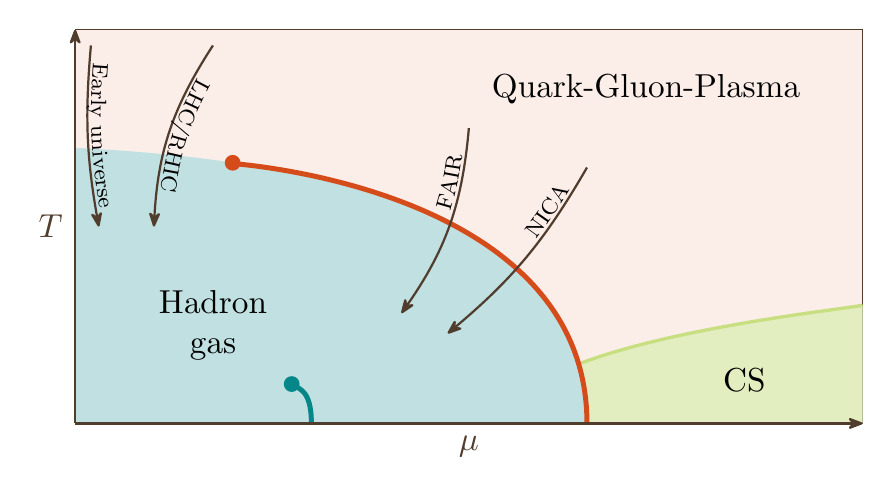
\begin{tikzpicture}

  \fill[ColourHl1, opacity=0.10] (0,0) rectangle (10cm,5cm);

  \draw[very thin, ColourDark] (0,0) rectangle (10cm,5cm);

  \fill[white, postaction={fill=ColourHl2, opacity=.25}]
    (5.5cm,0) ..controls +(0,1cm) and +(190:.5cm) .. (10cm,1.5cm)
    --(10cm,0) --cycle;

  \draw[ColourHl2!50, line width=1.2pt]
    (5.5cm,0) ..controls +(0,1cm) and +(190:.5cm) .. (10cm,1.5cm);

  \fill[white, line width=1.8pt, postaction={fill=ColourBase,opacity=0.25,}]
    (6.5cm, 0cm) .. controls +(0,3cm) and +(2cm,-.1cm) .. (0cm, 3.5cm)
    -- (0,0) -- cycle;

  \draw[ColourHl1, line width=1.8pt, shorten >=2cm]
    (6.5cm, 0cm) .. controls +(0,3cm) and +(2cm,-.2cm) .. (0cm, 3.5cm)
    node[shift={(2cm,-.19cm)},fill=ColourHl1, circle, inner sep=0pt, minimum size=.2cm] {};

  \draw[ColourBase, line width=1.8pt]
    (3cm, 0cm) .. controls +(0,.45cm) and +(320:0.1cm) .. (2.75cm,0.5cm)
    node[fill=ColourBase, circle, inner sep=0pt, minimum size=.2cm] {};

  \draw[thick,ColourDark,-{Stealth[round]}] (0,0) -- (10.0cm,0)
    node[midway, below,scale=1.2] {$\mu$};
  \draw[thick,ColourDark,-{Stealth[round]}] (0,0) -- (0, 5cm)
    node[midway, left,scale=1.2] {$T$};

  \node[scale=1.2] at (1.75cm,1.25cm) [align=center] {Hadron\\gas};
  \node[scale=1.2] at (7.25cm, 4.25cm)  {Quark-Gluon-Plasma};
  \node[scale=1.2] at (8.5cm,0.55cm)  {CS};

  \draw[
    thick,ColourDark,-{Stealth[round]},
    postaction={decorate,decoration={text along path, text align=center, text={|\footnotesize|Early universe}, raise=.3ex}},
  ] (0.2cm, 4.8cm) to [bend right=7.5] (0.3cm,2.5cm);

  \draw[
    thick,ColourDark,-{Stealth[round]},
    postaction={decorate,decoration={text along path, text align=center, text={|\footnotesize|LHC/RHIC}, raise=.3ex}},
  ] (1.75cm, 4.8cm) to [bend right=15] (1cm,2.5cm);

  \draw[
    thick,ColourDark,-{Stealth[round]},
    postaction={
      decorate,
      decoration={
        text along path,
        text align={right, right indent=0.35cm},
        text={|\footnotesize|FAIR},
        raise=.3ex,
        reverse path
      }},
  ] (5cm, 3.75cm) to [bend left=15] +(250:2.5cm);


  \draw[
    thick,ColourDark,-{Stealth[round]},
    postaction={
      decorate,
      decoration={
        text along path,
        text align={right, right indent=0.35cm},
        text={|\footnotesize|NICA},
        raise=.3ex,
        reverse path
      }},
  ] (6.5cm, 3.25cm) to [bend left=10] +(230:2.75cm);

  
\end{tikzpicture}
\end{document}


